\section{Source/Drain junctions}
As junction thickness decreases, the series resistance of the junction increases.
This cannot be neglected for conventional shallow junction technologies.

\begin{figure}[H]
	\centering
	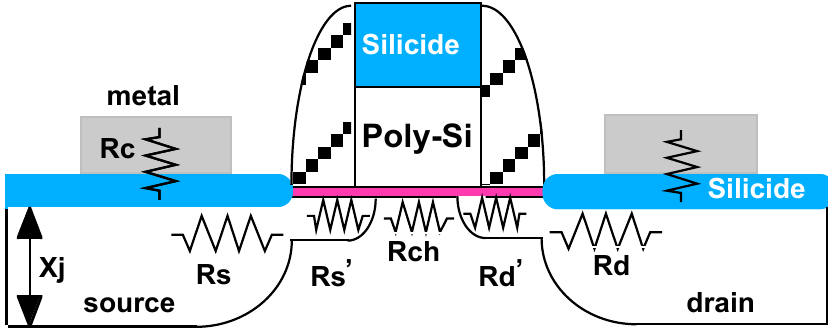
\includegraphics[scale=0.5]{junction_dimensioning1.png}
	\caption{Cross section with resistivities}
\end{figure}

Sheet resistance is given by
\begin{equation}
R_{sh}
=
\frac{\rho_s S}{W}
\end{equation}

Where the sheet resistivity is
\begin{equation}
\rho_s
=
\frac{\rho}{x_j}
\propto
\frac{1}{N_{sd} x_j}
\end{equation}

The channel resistance can be approximated by
\begin{equation}
R_{ch}
\propto
\frac{L_{ch} t_{ox}}{V_{gs}-V_{th}}
\end{equation}

As $L_g$ scales down
\begin{itemize}
	\item $R_{ch}$ scales down
	\item $R_{sd}$ does not scales as maximum doping is limited by solid solubility
	\item $R_{sd}$ becomes comparable to $R_{ch}$
	\item An increase in $R_{sd}$ becomes an important factor for device current
	\item Parasitic portion of the device is now playing important role in device performance and CMOS scaling
\end{itemize}
